\section{From a quoting certificate to an executable message policy}
\label{sec:productionquoting}

An academic benchmark and a production policy differ through their state,
action, observation and implementation contracts. Continuous time is not
itself the obstruction: a continuous-time jump process can retain integer
shares and tick prices. Nor does a Hawkes model impose independent arrivals;
its purpose is to represent excitation and temporal dependence
\citep{DeployBacry2015}. This section makes the additional contracts explicit
and derives a finite-action implementation certificate.

\subsection{A joint law for messages, fills and price marks}

At a local decision time $t$, let $\mathcal G_t$ contain only fully available
market data, reconciled private reports and prior sent messages. A sufficient
state can include tick spread, tagged ranks, inventory, outstanding buy and
sell reservations, pending requests, flow features, signal age and a posterior
for hidden regime or liquidity. The control is a native message, selected
from a finite feasible set: retain, cancel, replace, submit at an allowed
tick and size, or take liquidity. The action mask also enforces price,
inventory and message-budget constraints.

The required conditional law is jointly over fill times, executed quantities,
execution prices, fees, subsequent price marks, effective cancellation,
private-report arrival and next observation. Cancellation effectiveness and
its report time are distinct. A local cancel request stops neither fills nor
inventory risk by definition. State-dependent congestion can couple a delayed
cancel to precisely those events that make its order unattractive. Such a law
is covered by an augmented-state kernel, not by multiplying independent
marginal latency and toxicity distributions.

Maintain $q+o^b\le Q_{\max}$ and $q-o^a\ge-Q_{\max}$, where $o^b,o^a$
include unresolved submissions and requests that can leave orders executable.
A buy fill of $f$ changes $(q,o^b)$ to $(q+f,o^b-f)$, preserving the first
sum and relaxing the second bound; a sell fill has the symmetric property.
A cancel request does not release the reservation. This gives a pathwise
inventory invariant provided reports are reconciled and terminal release is
authoritative. A risk layer that merely refuses to count a real fill at a
boundary is not an inventory constraint.

Nasdaq's public ITCH book and private OUCH lifecycle have different roles
\citep{DeployITCH,DeployOUCH}. An order-by-order feed does not expose hidden
resting orders or the dealer's complete private state. A simulated FIFO
rank is exact only within the declared visible queue and arrival convention.
NYSE's parity allocation requires a different transition map
\citep{DeployNYSE}. Exchange-specific matching, repricing and replacement
rules must therefore be versioned inputs to the model.

\subsection{Ticks and implementation certificates without smoothness}

Fix a state and decision horizon. Let $Q(a)$ be the true action value with
one common continuation policy or optimal continuation, and let $s(a)$ be
the score actually computed by the implementation for each feasible message.
Suppose $|Q(a)-s(a)|\le e(a)$. The bounds may differ by message.

\begin{lemma}[Certified message selection]
\label{prop:compiledmessage}
For any emitted feasible action $\widetilde a$,
\begin{equation}\label{eq:compiledgap}
 \max_a Q(a)-Q(\widetilde a)
 \le \max_a\{s(a)+e(a)\}-\{s(\widetilde a)-e(\widetilde a)\}.
\end{equation}
For a baseline action $a_0$, its one-step advantage satisfies
\begin{equation}\label{eq:compiledadvantage}
 Q(\widetilde a)-Q(a_0)
 \ge s(\widetilde a)-s(a_0)-e(\widetilde a)-e(a_0).
\end{equation}
If all errors are at most $e$ and the emitted action is within $\xi$ of
maximizing $s$, its loss is at most $2e+\xi$. If one score exceeds all others
by more than $2e$, its exact maximizing action is identified.
\end{lemma}
\begin{proof}
Bound each competing value above by its score plus its error, and the emitted
value below by its score minus its error. Subtraction proves the first claim.
Reverse the two bounds for the baseline comparison. The uniform bound and
strict-margin conclusion follow immediately.
\end{proof}

This result applies to integer ticks and discrete order instructions with
no differentiability assumption. For a dynamic guarantee, choose the common
continuation as the fitted optimal value and insert the resulting local
loss into \citet[Theorem~39.1]{NoguerAlonso2026Execution}, or use the earlier
baseline-policy performance identity with that baseline's continuation.
A myopic score against a zero continuation cannot certify improvement of
an infinite-horizon inventory policy.

A deployable score enclosure may combine verified interpolation error,
fixed-point arithmetic error, model/continuation error and feature staleness.
For example, if the score is $L_a$-Lipschitz in a numerical feature $z$, its
stored representative $\bar z$ satisfies $\|z-\bar z\|\le h$, and arithmetic
error is at most $\nu_a$, these components contribute $L_a h+\nu_a$.
This statement does not apply across unmodeled changes of queue rank or
admissibility. Such branches must be enumerated or enclosed separately.
Integer arithmetic also needs a proved range that excludes overflow;
a mathematical quantization tolerance alone does not establish it.

If an omitted event set has conditional probability at most $p_{\rm tail}$
and action payoff on it has absolute error at most $D$, add
$Dp_{\rm tail}$ to the expected-score allowance. For unbounded losses one
instead needs an integrable tail bound, for example
$\E[|\text{error}|1_{\rm tail}]$. Quoting a measured latency percentile
without either allowance does not bound expected policy loss.

\subsection{The economic value of latency tails}

\begin{proposition}[Mean latency does not determine expected loss]\label{prop:latency-tail}
A resting order incurs loss $L>0$ if it is still live when an adverse trade
arrives at a fixed time $\tau>0$, and has no other payoff. A cancellation
effective exactly at $\tau$ is processed before that trade. Its cancellation
becomes effective at an independent delay $D\ge0$ with $\mathbb ED=m$, where
$0<m<\tau$. Then the expected loss is $L\Pr(D>\tau)$, and over all such laws
\[
  \bigl\{L\Pr(D>\tau):\ D\ge0,\ \mathbb ED=m\bigr\}=[0,\,Lm/\tau).
\]
The value $0$ is attained by the constant delay $D\equiv m$; the supremum is
approached by two-point laws on $\{0,\tau+\epsilon\}$ and is not attained.
\end{proposition}

\begin{proof}
The order is live at $\tau$ exactly when $D>\tau$. If $\Pr(D>\tau)>0$ then
$m\ge\mathbb E[D\mathbf 1_{\{D>\tau\}}]>\tau\Pr(D>\tau)$, so
$\Pr(D>\tau)<m/\tau$. The law putting mass $m/(\tau+\epsilon)$ at
$\tau+\epsilon$ and the rest at zero has mean $m$ and
$\Pr(D>\tau)=m/(\tau+\epsilon)\to m/\tau$. The set of laws with mean $m$ is
convex and the probability is linear in the law, so the attainable set is an
interval containing $0$ and all values below $m/\tau$.
\end{proof}
In the cell with loss $L=3$ ticks, adverse trade at $\tau=2$ and mean delay
$m=0.5$, the constant delay gives $0$, the mixture of $0.1$ (probability $0.9$)
and $4.1$ gives expected payoff $-0.3$ ticks (loss $0.3$ ticks), and delays with the same mean can reach losses
arbitrarily close to $0.75$ ticks. Clock units are synthetic.

More generally, for an adverse trade at time $\tau$ with fixed loss $L>0$
and no other payoff, the expected loss is
$L\mathbb P(D>\tau)$ under the specified joint law. If $\tau$ is random
and correlated with $D$, the probability is joint; replacing it by an
independent-latency calculation changes the model. The earlier phase-type
expansion remains useful under its assumptions, while this simple tail
example identifies an effect that moment matching alone cannot control.

FPGA acceleration is one implementation option, not a theorem hypothesis.
The relevant engineering record is the complete latency path: receipt,
decode, feature update, risk check, policy evaluation, serialization,
transport, exchange processing and private-report return. Tail behavior
under bursts and degraded conditions matters alongside central tendency.
A lookup can be constant in operation count while cache misses, contention
or queueing make wall-clock delay variable. Expensive estimation and
optimization may run outside the order-response path, provided the cached
policy's age and approximation errors remain in its declared envelope.

\subsection{Calibration with competing events and policy selection}

For a tagged order, log its entry context, size, rank estimate, message
history, every partial fill, effective terminal event and subsequent markouts.
A simplified cause-specific likelihood with observed at-risk indicator $Y_t$
and event hazards $\lambda_j(t\mid\mathcal G_{t-},a)$ is
\[
 \ell=\sum_j\int\log\lambda_j(t)\,\mathrm dN_j(t)
       -\int Y_t\sum_j\lambda_j(t)\,\mathrm dt.
\]
This is a counting-process likelihood under its declared conditional hazards,
not an instruction to discard unfilled orders. A cancellation is an observed
competing lifecycle event for the deployed policy. Estimating the hypothetical
fill time had the order not been canceled additionally requires conditional
censoring assumptions and support for remaining at risk. Conditioning only
on filled orders estimates a selected population and cannot identify an
unconditional fill hazard.

Model assessment should check fill time, partial volume, price mark and
cancellation exposure jointly across supported quote actions. Calibration
near a replacement boundary is especially consequential because small value
errors can change a discrete message. Use chronological holdouts and explicit
regime or drift allowances; do not apply an independent-sample confidence
formula to a clustered event stream without justification. The finite
calibration construction in Section~\ref{sec:deploymentcalibration} states
one sufficient sampling experiment and an explicit unsupported-row rule.

\subsection{Reference implementation and falsification cases}

The code emits a normalized event trace with exchange and receipt times,
tracks a tagged FIFO queue through adds, cancels ahead/behind and partial
consumption, and retains executable exposure until cancellation is effective
and privately resolved. It exercises the following failure cases: treating
a cancel request as terminal, releasing exposure before reconciliation,
using a future exchange event before receipt, double-counting a report,
changing quote price without accounting for lost rank, and choosing a
compiled message whose score margin is smaller than its error allowance.

\begin{table}[htbp]
\centering\small
\caption{Synthetic quoting checks. Payoffs are ticks per declared order;
clock units are arbitrary. The mean delay is identical in the two rows.}
\begin{tabular}{p{.57\linewidth}r}
\toprule
Quantity & Value\\\midrule
\inputtable{tables/production_rows.tex}
\bottomrule
\end{tabular}
\end{table}

The independent policy evaluation tests do not assume the selected action
is optimal. They compute its value under the test law and compare its loss
with the certificate. Message conformance, real latency measurements,
borrow/funding access, actual fee tiers and production incident recovery
remain external evidence requirements. The mathematical completion here is
an explicit model-to-implementation contract with reproducible checks,
not an assertion of a profitable exchange-connected market maker.


\begin{figure}[htbp]
\centering
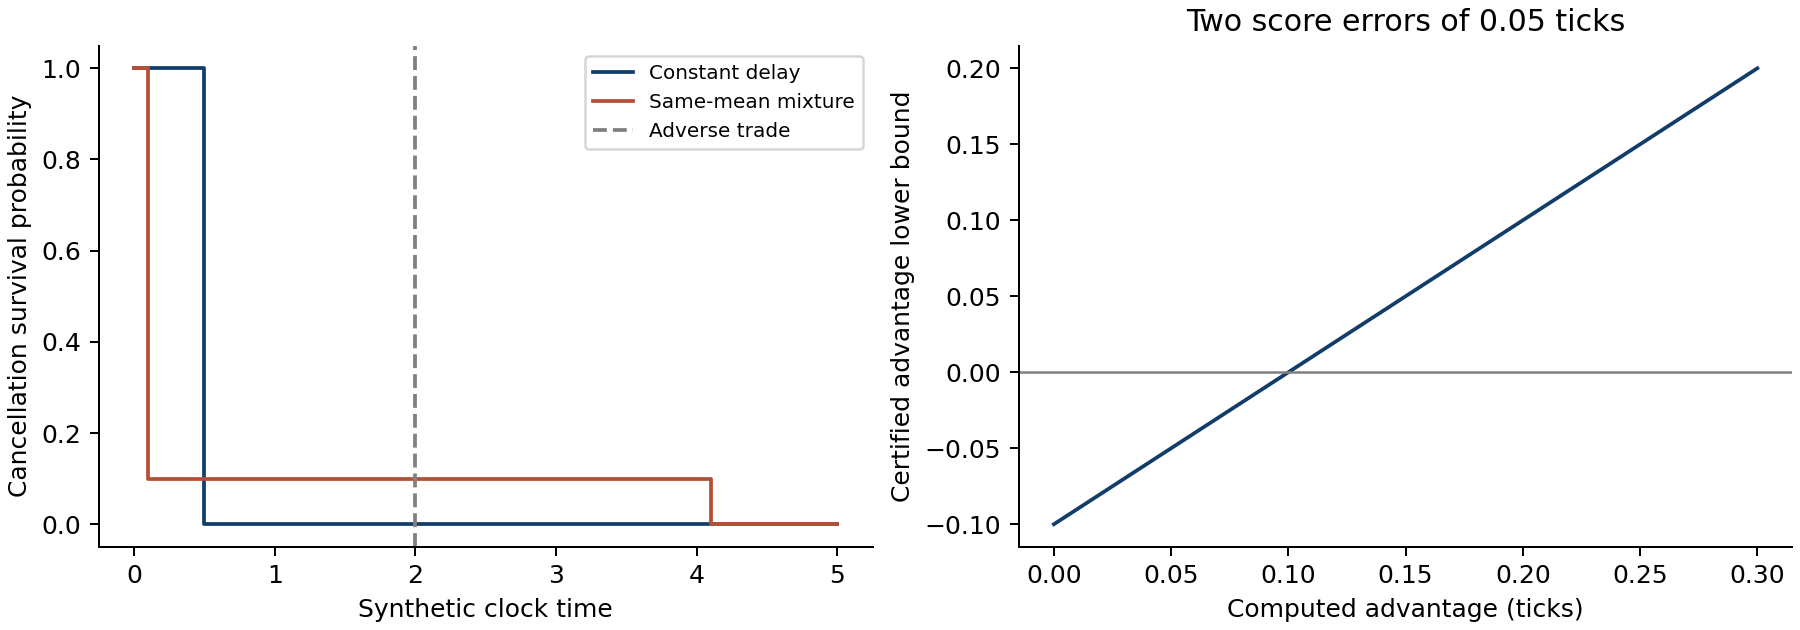
\includegraphics[width=\linewidth]{figures/07_production_bridge.png}
\caption{Discrete implementation diagnostics generated by the accompanying
reference suite. All axes use synthetic model units; the curves illustrate
the declared mechanisms rather than estimated market behavior.}
\label{fig:productionbridge}
\end{figure}

\subsection{Persistence, competition and the scope of the dealer law}
The event rates of Assumption~\ref{ass:finite} depend on the observable state $(q,z,a)$, so
persistent flow enters only through the regime coordinate $z$. The
switching-friction mechanism of \citet{RodriguezDominguez2026Switching} predicts
execution-weighted duration restrictions that a stationary two-regime chain, as in Section~12.5, cannot reproduce
asymptotically. A finite-window approximation must be justified and its
error charged; enlarging a finite state alone does not create true
asymptotic long memory. The equilibrium
conclusions of \citet{RodriguezDominguez2026Market} rest on timing restrictions that
differ from ours, since the conditional fill--price marks here can represent
informed flow. Their relevance is to the family $\Theta$ of Theorem~\ref{thm:baselinequoting}, which is
fixed: if rivals come to condition on the same representation, $\Theta$ must
contain the law after that adoption, not before it.

